\documentclass[tikz]{standalone}
%\usetikzlibrary{positioning}
\usetikzlibrary{decorations.pathmorphing}
\usetikzlibrary{decorations.markings}
\usetikzlibrary{shapes.misc}
\usetikzlibrary{intersections}
\usetikzlibrary{arrows}
\tikzset{>={latex}}
\tikzstyle{X}=[cross out, draw, orange, scale = 0.75, thick]

\begin{document}
		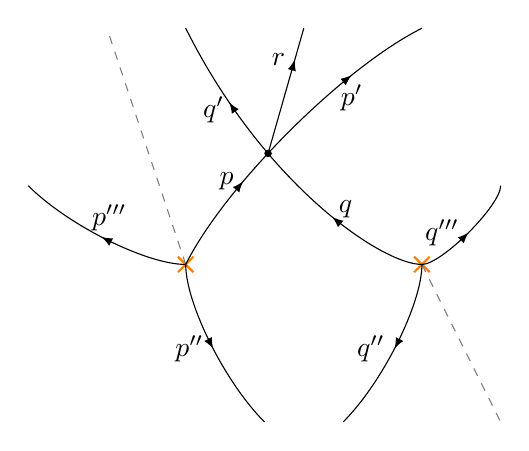
\begin{tikzpicture}[scale=1]
			%\draw [help lines] (-2,-2) grid (4,3);
	
			\node[X] at (0,0) {};
			%\node[right, orange] at (0,0) {$\alpha$};
	        \draw[dashed, gray] (0,0) -- (-1,3);
	
			\draw[
				decoration={markings, 
					%mark = at position 0.9 with {\node[above] {A};},			
					mark = at position 0.5 with {\arrow[scale=1]{>}},
					mark = at position 0.5 with {\node[left]{$p''$};}
				},
	        	postaction={decorate}
	        ] (0,0) .. controls (0,-.5) and (.5, -1.5) .. (1,-2);
	   		\draw[
				name path = S12,
				decoration={markings, 
					%mark = at position 0.9 with {\node[above] {B};},			
					mark = at position 0.3 with {\arrow[scale=1]{>};},				
					mark = at position 0.3 with {\node[left]{$p$};},
					mark = at position 0.75 with {\arrow[scale=1]{>};},				
					mark = at position 0.75 with {\node[below]{$p'$};}
				},
		       	postaction={decorate}
	        ] (0,0) .. controls (.5,1) and (2,2.5) .. (3,3);
			\draw[
				decoration={markings, 
					%mark = at position 0.9 with {\node[above] {C};},						
					mark=at position 0.5 with {\arrow[scale=1]{>}},
					mark = at position 0.45 with {\node[above]{$p'''$};}
				},
	        	postaction={decorate}
	        ] (0,0) .. controls (-0.5,0) and  (-1.5,0.5) .. (-2,1);
			
			\node[X] at (3,0) {};
			%\node[below left, orange] at (3,0) {$\beta$};		
	        \draw[dashed, gray] (3,0) -- (4,-2);		
	
			\draw[
				name path = S23,
				decoration={markings, 
					mark = at position 0.3 with {\arrow[scale=1]{>}},
					mark = at position 0.25 with {\node[above]{$q$};},
					mark = at position 0.75 with {\arrow[scale=1]{>}},
					mark = at position 0.725 with {\node[left]{$q'$};}
				},
	        	postaction={decorate}
	        ] (3,0) .. controls (2.5,0) and  (1,1) .. (0,3);
			\draw[
				decoration={markings, 
					mark = at position 0.5 with {\arrow[scale=1]{>}},
					mark = at position 0.5 with {\node[left]{$q''$};}
				},
	        	postaction={decorate}
	        ] (3,0) .. controls (3,-.5) and (2.5, -1.5) .. (2,-2);
			\draw[
				decoration={markings, 
					mark = at position 0.5 with {\arrow[scale=1]{>}},
					mark = at position 0.5 with {\node[left]{$q'''$};}
				},
	        	postaction={decorate}
	        ] (3,0) .. controls (3.25,0) and (4, 0.75) .. (4,1);
	
	
			\path[name intersections = {of = S12 and S23, by = {joint123}}];
			
			\draw [
				decoration={markings, 
					mark = at position 0.75 with {\arrow[scale=1]{>}},
					mark = at position 0.75 with {\node[left]{$r$};}
				},
	        	postaction={decorate}
			] (joint123) -- (1.5,3);

	        \draw[fill] (joint123) circle (.04);	
	        
		\end{tikzpicture}
\end{document}